\section{Evaluation}
\label{sec:eval}

Our evaluation aims to answer the following questions:
\begin{itemize}[leftmargin=0.9em,labelsep=0.35em]
  \item Can \system retain work in microbenchmarks?~(\S\ref{sec:eval-causal})
  \item Can \system reduce real-world token use?~(\S\ref{sec:eval-agent})
  \item Can \system reduce real-world workflow time?~(\S\ref{sec:eval-time})
  \item Can \system reduce agent-execution time?~(\S\ref{sec:eval-mechanisms})
  \item Can \system limit replay and recovery costs?~(\S\ref{sec:eval-replay})
  \item Can \system keep filesystem overhead low?~(\S\ref{sec:eval-file-commit})
\end{itemize}

\begin{figure*}[t]
  \centering
  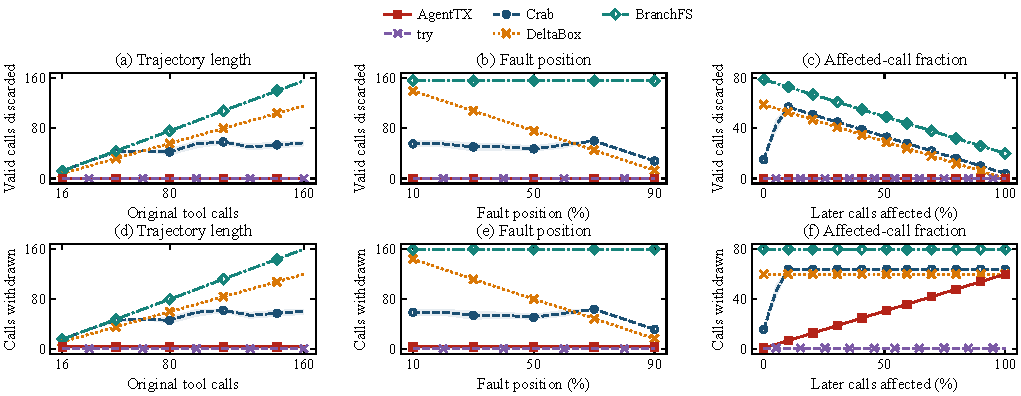
\includegraphics[width=\linewidth]{FIG-System-Micro-Recovery.pdf}
  \caption{\textbf{Recovery scope on fixed command trajectories.}
  \small\emph{Top: valid calls discarded. Bottom: total calls withdrawn.
  Columns vary trajectory length, fault position, and the fraction of later
  calls affected. Each sweep point averages ten cases with three
  repetitions each; bands show 95\% case-bootstrap intervals.
  Recovery completeness is reported in Table~\ref{tab:controlled-policy-results}.}}
  \label{fig:system-micro-recovery}
\end{figure*}

\subsection{Setup and Methodology}
\label{sec:eval-setup}

\textbf{Testbed.}
We run the experiments on a server with two 32-core Intel Xeon Gold 6530
CPUs and 128\,GiB DRAM, running Ubuntu 24.04 with Linux kernel
6.8.0-147. Recovery workloads execute in containers using OverlayFS over
Ext4, with \texttt{strace} recording file accesses.

\textbf{Baselines.}
We compare \system with Crab, DeltaBox, BranchFS, and \trycmd, implementing their
Table~\ref{tab:granularity} recovery scopes on the common OverlayFS runtime
as in Section~\ref{sec:motivation-observations}.
For storage overhead, we compare \system with OverlayFS, \trycmd,
DeltaBox~\cite{deltabox}, and BranchFS~\cite{branchfs} on Ext4 and XFS, using the native filesystem
as the direct-update reference.

\textbf{Methodology.}
Scripts execute the fixed command trajectories, repeating each case three
times. Real-world experiments use SWE-agent and Codex on
SWE-Bench Lite~\cite{swebench} and Terminal-Bench~\cite{tbench}.
Both agents use GPT-5.6 Luna with maximum reasoning effort. \system uses
compact agent context, while the real-world competitors use full context.

\textbf{Recovery input and measurement scope.}
The file-report protocol gives \system the user-specified file and a
reference checkpoint, defaulting to the committed boundary. Controls retain
exact step hints; Crab also receives the affected turns. The recovery
measurements below were collected with the earlier verifier-guided selector.
They measure recovery scope and cost; a full rerun with file reports is
pending.

\subsection{RQ1: Microbenchmarks}
\label{sec:eval-causal}

We reuse the 400 fixed trajectories from
Section~\ref{sec:motivation-observations}: 100 vary trajectory length, 90
fault position, and 210 the fraction of later calls affected by the fault.
Scripts execute each trajectory under \system, Crab, DeltaBox,
BranchFS, and \trycmd, with three repetitions per method, totaling
6,000 runs. Each run executes the trajectory and
applies recovery using the shared runtime. \system is not given the injected fault
step or affected-call set. These recorded runs use the earlier selector
with captured dependencies and verifier feedback, while the competitors attain the best
valid-work retention permitted by their policies, with exact fault-location
hints where needed.
Injection records supply ground truth for scoring error
removal and independent-work retention. These checks run at the recovery
boundary without model calls, independently of subsequent task success.

\begin{table}[!ht]
\centering
\caption{\textbf{Error removal and valid-work retention.}
\small\emph{Each method has 1,200 fixed-trajectory runs. Percentages and
call counts are averaged over runs.}}
\label{tab:controlled-policy-results}
\footnotesize
\setlength{\tabcolsep}{2pt}
\begin{tabular*}{\linewidth}{@{\extracolsep{\fill}}lrrrr@{}}
\toprule
Method & \shortstack{Affected\\removed} & \shortstack{Valid\\retained} & \shortstack{Valid\\discarded} & \shortstack{Calls\\withdrawn} \\
\midrule
\system & 100\% & 100\% & 0.00 & 17.93 \\
try & 17.03\% & 100\% & 0.00 & 1.00 \\
Crab & 100\% & 45.98\% & 38.12 & 56.04 \\
DeltaBox & 100\% & 43.10\% & 48.18 & 66.10 \\
BranchFS & 100\% & 0\% & 82.08 & 100.00 \\
\bottomrule
\end{tabular*}
\end{table}


\textbf{Error removal.}
Table~\ref{tab:controlled-policy-results} shows that \system, Crab,
DeltaBox, and BranchFS remove all affected calls in every run, giving
1,200 complete recoveries per method. \trycmd removes 17.03\% of affected
calls on average and completes recovery in 30 of 1,200 runs (2.5\%).

\textbf{Independent work retained.}
Table~\ref{tab:controlled-policy-results} shows that \system retains all
independent work. Crab, DeltaBox, and BranchFS
retain 45.98\%, 43.10\%, and 0\%, respectively. They discard an average
of 38.12, 48.18, and 82.08 valid calls per run, compared with zero for
\system. Including affected calls, the corresponding withdrawal counts
are 56.04, 66.10, and 100.00, versus 17.93 for \system.
\trycmd retains all independent work but withdraws only one call per run,
leaving dependent effects in the other 97.5\% of runs.
Selecting affected calls preserves independent progress that the other
complete-recovery policies discard.

\textbf{Effect of trajectory structure.}
In Figure~\ref{fig:system-micro-recovery}(a,d), trajectory length grows
while the affected set stays at four calls. At 160 calls, Crab,
DeltaBox, and BranchFS withdraw 60.8, 120, and 160 calls,
while \system withdraws four. In Figure~\ref{fig:system-micro-recovery}(b,e),
moving the fault from 10\% to 90\% of a 160-call trajectory reduces
the number of calls withdrawn by DeltaBox from 144 to 17; \system still
withdraws four. In Figure~\ref{fig:system-micro-recovery}(c,f), the
affected fraction increases in 80-call trajectories. The number withdrawn by \system grows
from one to 60 calls as dependencies spread, while DeltaBox
continues to withdraw 60. The top row shows that \system discards no
independent calls throughout these sweeps. The \trycmd scope remains at one
call even as the affected set grows.

\subsection{RQ2: Real-World Token Cost}
\label{sec:eval-agent}

\textbf{Workloads and setup.}
We evaluate all 300 SWE-Bench Lite tasks~\cite{swebench} and 241
Terminal-Bench tasks~\cite{tbench} with SWE-agent and Codex under the settings
in Section~\ref{sec:eval-setup}. Each run executes a scripted fault prefix,
applies a recovery policy,
regenerates discarded notes, and lets the agent complete the original task.
These recorded runs use the earlier selector and hints described in
Section~\ref{sec:eval-causal}; each injected-prefix call occupies its own
turn. SWE injection targets gold-patch file paths, which can appear in the
recovery handoff.

Token comparisons use tasks that succeed
under both methods and have complete costs; SWE \trycmd pairs use task-test
success. We match tasks, images, model,
fault seed, recovery contract, and budgets, pooling infrastructure variants
for Crab and \trycmd. Token totals use API-reported usage, including replay and all
recorded attempts. For token cost $C$, savings are
$100(1-\sum C_{\mathrm{Lancet}}/\sum C_{\mathrm{control}})$; 95\%
intervals use 20,000 paired task-bootstrap samples within configuration
strata.

\begin{table}[!ht]
\centering
\caption{\textbf{Task successes on real-world tasks.}
\small\emph{Successful tasks pass the target SWE tests or official TB verifier.
Counts cover 300 SWE
and 241 TB tasks.}}
\label{tab:swe-full-results}
\footnotesize
\setlength{\tabcolsep}{3pt}
\begin{tabular*}{\linewidth}{@{\extracolsep{\fill}}lrrrr@{}}
\toprule
 & SWE & SWE & TB & TB \\
Method & SWE-agent & Codex & SWE-agent & Codex \\
\midrule
\system & 285 & 288 & 208 & 223 \\
Crab & 272 & 284 & 188 & 206 \\
DeltaBox & 288 & 290 & 206 & 224 \\
BranchFS & 248 & 282 & 209 & 227 \\
\trycmd & 187 & 229 & 202 & 220 \\
\bottomrule
\end{tabular*}
\end{table}


\textbf{Task outcomes.}
Table~\ref{tab:swe-full-results} reports task success. With SWE-agent and
Codex, respectively, \system achieves success rates of 95.0\% and 96.0\% on
SWE-Bench Lite, and 86.3\% and 92.5\% on Terminal-Bench.

\begin{figure}[t]
  \centering
  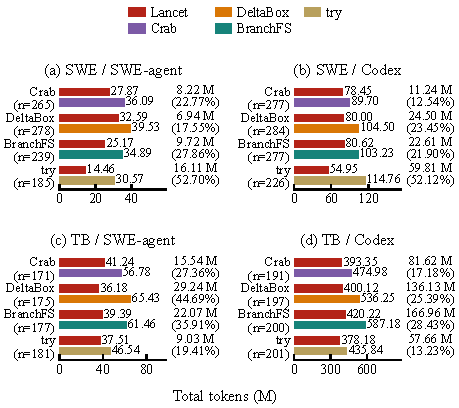
\includegraphics[width=\linewidth]{FIG-Realworld-Token-Savings.pdf}
  \caption{\textbf{Token totals and savings on control-specific matched tasks.}
  \small\emph{Paired bars show total tokens on matched successful tasks;
  $n$ counts pairs. Right labels give savings in millions (M) and percent.
  Task sets differ between controls; token scales differ between panels.}}
  \label{fig:realworld-token-savings}
\end{figure}

\textbf{Model cost.}
Figure~\ref{fig:realworld-token-savings} shows that \system saves
17.55--44.69\% relative to DeltaBox and 21.90--35.91\% relative
to BranchFS across the four benchmark/agent combinations.
Against Crab, savings are 22.77\%, 12.54\%, 27.36\%, and
17.18\% on SWE/SWE-agent, SWE/Codex, TB/SWE-agent, and TB/Codex,
respectively.
For scale, the 175 TB/SWE-agent pairs against DeltaBox consume
36.18 million Lancet tokens versus 65.43 million control tokens, a
44.69\% reduction.
Against \trycmd, savings are 52.70\%, 52.12\%, 19.41\%, and 13.23\%
on the same four benchmark/agent combinations, using 185, 226, 181,
and 201 matched pairs, respectively.

\textbf{Answer to RQ2.}
Across SWE-Bench Lite and Terminal-Bench with both agents, \system
reduces total token use on matched tasks by
12.54--52.70\% across the evaluated controls.

\subsection{RQ3: Real-World Workflow Time}
\label{sec:eval-time}

We measure workflow time on the same task pairs as
Section~\ref{sec:eval-agent}, using the same cost-ratio formula for savings.
Workflow time subtracts the entire localization stage, including initial
error checks and candidate search and validation, overlapped with agent
execution from recorded elapsed time. It retains setup, plan application,
replay, model execution, and final verification across all attempts,
excluding queue time.

\begin{figure}[t]
  \centering
  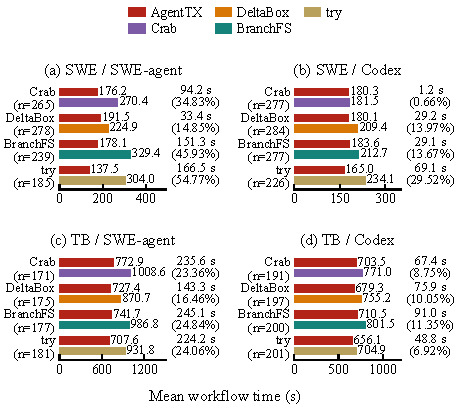
\includegraphics[width=\linewidth]{FIG-Realworld-Time-Savings.pdf}
  \caption{\textbf{Workflow time and savings on matched tasks.}
  \small\emph{Paired bars show mean workflow time on the same task pairs as
  Figure~\ref{fig:realworld-token-savings}; $n$ counts pairs. Right labels
  give mean seconds saved per task and percentage savings.}}
  \label{fig:realworld-time-savings}
\end{figure}

Figure~\ref{fig:realworld-time-savings} shows that, relative to DeltaBox,
mean time falls from 224.92\,s to 191.52\,s
on SWE/SWE-agent, from 870.70\,s to 727.40\,s on TB/SWE-agent, and from
755.19\,s to 679.28\,s on TB/Codex. These correspond to reductions of
14.85\%, 16.46\%, and 10.05\%, respectively. On SWE/Codex, mean time falls from
209.40\,s to 180.15\,s, a 13.97\% reduction.
Relative to BranchFS, time falls by 45.93\%, 13.67\%, 24.84\%, and
11.35\% on SWE/SWE-agent, SWE/Codex, TB/SWE-agent, and TB/Codex,
respectively.
Relative to Crab, Lancet reduces mean time from 270.41 to
176.23\,s on SWE/SWE-agent (34.83\%) and from
181.48 to 180.29\,s on SWE/Codex (0.66\%). TB/SWE-agent and TB/Codex show mean
reductions of 23.36\% and 8.75\%, respectively.
Against \trycmd, mean time falls from 304.03 to 137.51\,s on SWE/SWE-agent,
from 234.11 to 164.99\,s on SWE/Codex, from 931.83 to 707.61\,s on
TB/SWE-agent, and from 704.91 to 656.11\,s on TB/Codex: reductions of
54.77\%, 29.52\%, 24.06\%, and 6.92\%, respectively.

\textbf{Answer to RQ3.}
\system achieves lower mean workflow time in all 16 comparisons,
with reductions of 0.66--54.77\% across the two benchmarks and agents.

\subsection{Breakdown}
\label{sec:eval-breakdown}

Figure~\ref{fig:runtime-stage-cost} decomposes the matched runs and
workflow time from Section~\ref{sec:eval-time} into agent execution,
final verification, and setup/replay. Agent execution includes model
calls and tool use; verification measures final task grading.

\begin{figure}[t]
  \centering
  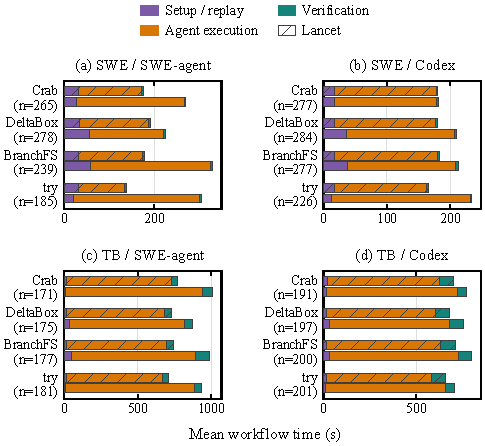
\includegraphics[width=\linewidth]{FIG-Realworld-Stage-Cost.pdf}
\caption{\textbf{Workflow-time breakdown on real tasks.}
  \small\emph{Pairs and time accounting match
  Figure~\ref{fig:realworld-time-savings}. Hatched bars show \system;
  solid bars show the named competitor. Colors distinguish stages;
  $n$ counts matched task pairs.}}
  \label{fig:runtime-stage-cost}
\end{figure}

% Queue the wide storage figure early to place it alongside the RQ6 analysis.
\begin{figure*}[t]
  \centering
  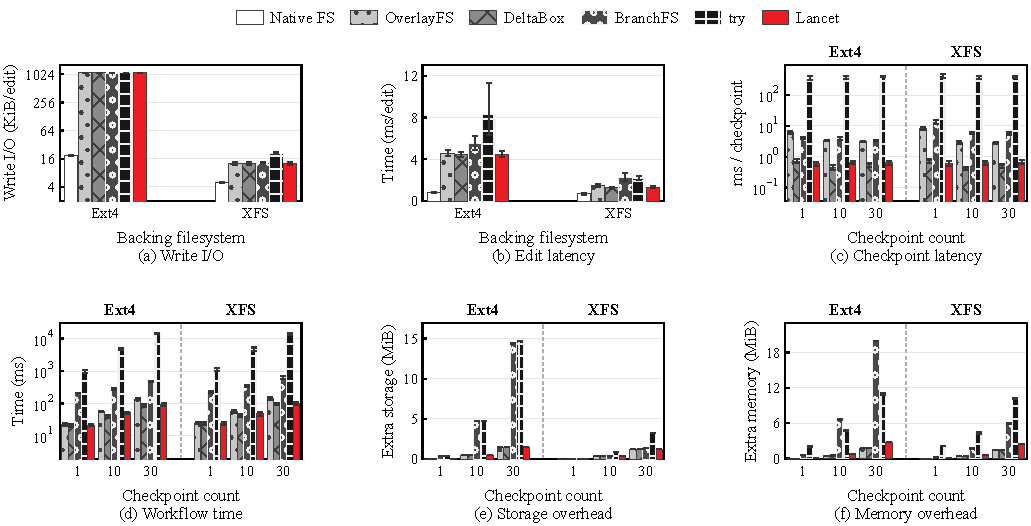
\includegraphics[width=\linewidth]{FIG-RQ5-Storage.pdf}
  \caption{\textbf{Filesystem costs.}
  (a) Write I/O; (b) synced edit latency; (c) checkpoint latency;
  (d) workflow time; (e) extra storage; (f) extra memory.
  Axes in (a), (c), and (d) use log scales.
  Bars show means with 95\% bootstrap intervals.}
  \label{fig:rq5-storage}
\end{figure*}

\subsubsection{RQ4: Agent Execution}
\label{sec:eval-mechanisms}

On SWE-Bench Lite (Figure~\ref{fig:runtime-stage-cost}(a--b)),
agent execution falls from 165.13 to 155.18\,s with SWE-agent and from
169.56 to 159.60\,s with Codex, relative to DeltaBox. Against Crab,
the SWE-agent execution stage falls from 238.99 to 140.86\,s,
while SWE/Codex has similar
execution times of 161.81 and 160.72\,s. Against \trycmd, agent execution
falls from 279.73 to 102.60\,s with SWE-agent and from 219.00 to
145.62\,s with Codex.

On Terminal-Bench (Figure~\ref{fig:runtime-stage-cost}(c--d)),
agent execution accounts for most of the time saved relative to DeltaBox:
it falls from 781.14 to 668.21\,s with SWE-agent and from 650.49 to
585.63\,s with Codex. Against \trycmd, it falls from 875.33 to 653.27\,s
with SWE-agent and from 652.11 to 562.18\,s with Codex.
Across all sixteen comparisons, agent execution
accounts for 74.6--92.3\% of \system workflow time.

\subsubsection{RQ5: Replay and Recovery}
\label{sec:eval-replay}

\subsection{RQ6: Storage and Checkpoint Costs}
\label{sec:eval-file-commit}

Figure~\ref{fig:rq5-storage} compares \system, OverlayFS, BranchFS~\cite{branchfs},
\trycmd~\cite{try-osdi26}, and the DeltaFS component of
DeltaBox~\cite{deltabox} on Linux 6.8.0-147, using 4\,GiB Ext4 and
reflink-enabled XFS volumes.
Native Ext4 and XFS provide direct-update references.
Partial-update tests perform five non-truncating 4\,KiB edits to a
1\,MiB file, retaining the initial version and checkpointing after each
edit. Block-device writes and edit latency include \texttt{syncfs} but
exclude the subsequent checkpoint. The remaining tests use 100 target
files and overwrite ten seed files, all 4\,KiB, before each of 1, 10,
or 30 checkpoints. For \trycmd, checkpoint timing includes saving an
environment, exiting, and reentering a new view.
Workflow time covers setup, buffered writes, checkpoints, publication,
and cleanup. We report twenty timing runs per configuration. Resource
overhead is the difference in growth from initialization to just before
publication between ten paired runs with and without checkpoints.
Storage counts shared extents once; memory includes anonymous pages,
file cache, and kernel allocations across all worker processes.

Figure~\ref{fig:rq5-storage}(a--b) shows that XFS reduces the data
copied for partial updates. On Ext4, \system writes 1,102.44\,KiB per
edit because copy-up copies the original file; XFS reflink shares
unchanged extents, reducing writes to 12.71\,KiB. Synced edit latency
falls from 4.496 to 1.331\,ms. On XFS, OverlayFS and DeltaBox write
12.71 and 12.73\,KiB with similar edit latency. Thus, the user-space
controller preserves the data-sharing benefits of the backing filesystem.

Figure~\ref{fig:rq5-storage}(c--d) shows the benefit of retaining mount
references during checkpoint creation. Across the tested depths,
\system takes 0.58--0.67\,ms per checkpoint, a 4.20--13.66$\times$
speedup over OverlayFS. At thirty checkpoints, complete workflows take
95.22\,ms on Ext4 and 99.22\,ms on XFS, reducing time by 30.8\% and
30.5\% relative to OverlayFS, and by 79.8\% and 84.3\% relative to
BranchFS. The corresponding \trycmd workflows take 14.159 and
13.958\,s. DeltaBox has lower repeated-checkpoint costs, taking
0.546 and 0.504\,ms per checkpoint at this depth on Ext4 and XFS.

Figure~\ref{fig:rq5-storage}(e--f) shows the resource cost of this
optimization. At thirty checkpoints, \system uses 1,524\,KiB of extra
storage on Ext4 and 1,284\,KiB on XFS, just 4\,KiB more than OverlayFS
and DeltaBox for generation records. Extra memory is 2,760.4 and
2,499.2\,KiB, respectively, about 1\,MiB above those two systems
because retained mount references keep kernel metadata live.
Both storage and memory remain below the corresponding BranchFS and
\trycmd costs. The main tradeoff is therefore additional resident
memory for faster checkpoints, with little extra storage.
